	\chapter{Detecting \ac{EWFO} on \ac{MAV}}
	\label{sec:object_detection}
	
	This chapter addresses the detection of \ac{EWFO}. In particular the following research questions are addressed:
	
\begin{enumerate}
	\item[\textbf{RQ2}]What kind of architecture is suitable to detect \acp{EWFO}?
	\item[\textbf{RQ3}]What are the trade-offs in detection performance and inference time when a detection model for \acp{EWFO} is deployed on a \ac{MAV}?
%	\item[\textbf{RQ4}]Can the gained insights be used to build a lightweight and robust detection model for racing gates in the \ac{IROS} Autonomous Drone Race?
\end{enumerate}

	The chapter introduces the model used for this work and conducts several experiments to find a suitable architecture.
	
	\section{Methodology}
	
	A literature review has been conducted in order to find a suitable approach for the detection of \ac{EWFO} on \acp{MAV}. \acp{CNN} achieve currently the best performance however, their drawback is their computational requirements and their need of data. We hypothesize that due to the simplicity of the object it is possible to generate training data using a graphical engine and to simplify the \acp{CNN} architecture to speed up the inference time.
	
	A trade-off between accuracy and inference speed are One-Stage Object Detectors such as \ac{Yolo} and \ac{SSD}. We decide for Yolo as a framework is available that simplifies the implementation on the target platform.
	
	The original training goal is defined as follows:
	\if false
	\begin{align}
	&\lambda_{coord} \sum_{i=0}^{S^2}\sum_{j=0}^B \mathbb{1}_{ij}^{obj}[(x_i-\hat{x}_i)^2 + (y_i-\hat{y}_i)^2 ] \\&+ \lambda_{coord} \sum_{i=0}^{S^2}\sum_{j=0}^B \mathbb{1}_{ij}^{obj}[(\sqrt{w_i}-\sqrt{\hat{w}_i})^2 +(\sqrt{h_i}-\sqrt{\hat{h}_i})^2 ]\\
	&+ \sum_{i=0}^{S^2}\sum_{j=0}^B \mathbb{1}_{ij}^{obj}(C_i - \hat{C}_i)^2 + \lambda_{noobj}\sum_{i=0}^{S^2}\sum_{j=0}^B \mathbb{1}_{ij}^{noobj}(C_i - \hat{C}_i)^2 \\
	&+ \sum_{i=0}^{S^2} \mathbb{1}_{i}^{obj}\sum_{c \in classes}(p_i(c) - \hat{p}_i(c))^2 \\
	\end{align}
	\fi
	
	\begin{equation}
	\mathcal{L} = \lambda_{loc}\mathcal{L}_{loc} + \lambda_{obj}\mathcal{L}_{obj} + \lambda_{noobj}\mathcal{L}_{noobj} + \lambda_{class}\mathcal{L}_{class}
	\end{equation}
	where $\mathcal{L}_{loc}$ is the target for bounding box regression, $\mathcal{L}_{obj}$ the loss where a object is present, $\mathcal{L}_{noobj}$ the loss where there is no object and $\mathcal{L}_{class}$ the classification loss. $\lambda$ are trade-off parameters between the multiple targets.
	
	For a single class prediction this can be simplified to:
	
	\begin{equation}
	\mathcal{L} = \lambda_{loc}\mathcal{L}_{loc} + \lambda_{obj}\mathcal{L}_{obj} + \lambda_{noobj}\mathcal{L}_{noobj}
	\end{equation}
	
	The object loss is defined as:
	
	\begin{equation}
		\mathcal{L}_{obj} = \sum_{i=0}^{S^2}\sum_{j=0}^B \mathbb{1}_{ij}^{obj}(\log(1+\exp(-o_{ij} \cdot \hat o_{ij}))
	\end{equation}
	where $o_{ij}$ is a softmax activation assigned to anchor box $i$,$j$,$\hat o_{ij}$ the ground truth label assigned to that box, 1 for object and -1 for no object.  $\mathbb{1}_{ij}^{obj}$ is 1 if the anchor box at $i$,$j$ is responsible to predict a certain object and 0 otherwise. The responsibility is determined by \ac{IoU} with a ground truth box. The box with the highest \ac{IoU} with the ground truth box gets assigned responsible.\todo{double check}
	
	The noobject loss is defined vice versa but triggered by the $\mathbb{1}_{ij}^{noobj}$ binary variable.
	
	The localization target is defined as:
	
	\begin{equation}
		\mathcal{L}_{loc} = \sum_{i=0}^{S^2}\sum_{j=0}^B \mathbb{1}_{ij}^{obj}[(x_{ij}-\hat{x}_{ij})^2 + (y_i-\hat{y}_{ij})^2  + (\sqrt{w_{ij}}-\sqrt{\hat{w}_{ij}})^2 +(\sqrt{h_{ij}}-\sqrt{\hat{h}_{ij}})^2 ]
	\end{equation}
	where $x$,$y$ are the center coordinates and $w$,$h$ are the bounding box width and height. $\mathbb{1}_{ij}^{obj}$ is 1 if the set of output nodes at $i$,$j$ is responsible to predict a certain object and 0 otherwise. 
	
	\section{Depth and Width}
	
	State of the art results of Computer Vision benchmarks are achieved by particularly deep/wide models. The vast amount of parameters and layers enables to model highly non-linear functions and complex image features. However, \acp{EWFO} do not contain very complex shapes. Instead the object parts are of thin structure and are spread across large parts of the image. Hence, we hypothesize that a very deep/wide network will not perform better than a shallower and thinner counterpart. Also, current feature extractors are designed to detect complex objects of multiple classes. In this work we investigate the single class case. We hypothesize that this requires less filters and thus that are thinner and shallower counterpart can detect the object with equal performance.
	
	\begin{figure}
		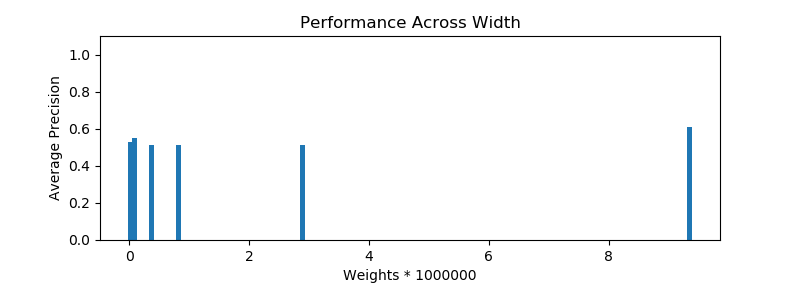
\includegraphics[width=\textwidth]{fig/perf_width}
	\end{figure}
	
	\section{Receptive Field}
	
		
	\section{Reducing Inference Time}
	
	\section{title}